\chapter{Συστήματα Συντεταγμένων}
\label{apx:coordinates}

\section{Καρτεσιανές συντεταγμένες}
Οι καρτεσιανές συντεταγμένες μας επιτρέπουν να προσδιορίσουμε τη θέση ενός σημείου στο επίπεδο, ή στον τριδιάστατο χώρο\footnote{Όλο το παράρτημα είναι μετάφραση της σελίδας \url{https://mathinsight.org/spherical_coordinates}, η οποία περιέχει και διάφορα applets για την καλύτερη κατανόηση των εννοιών.}. Οι καρτεσιανές συντεταγμένες (ή επίπεδες συντεταγμένες) ενός σημείου αποτελούνται από ένα ζεύγος αριθμών (στις δύο διαστάσεις) ή μια τριπλέτα αριθμών (στις τρεις διαστάσεις) που καθορίζουν την διανυσματική απόσταση από τον άξονα των συντεταγμένων.

\subsection{Καρτεσιανές συντεγαμένες στο επίπεδο}
Οι καρτεσιανές συντεταγμένες στο επίπεδο προσδιορίζονται με όρους των συντεταγμένων στους άξονες x και y, όπως φαίνεται στο παρακάτω σχήμα
(Σχήμα \ref{fig:apxA_cartesian2D}). Η αρχή των αξόνων ορίζεται ως το σημείο τομής των αξόνων x και y. Οι καρτεσιανές συντεταγμένες ενός σημείου του επιπέδου γράφονται ως (x,y). Ο πρώτος αρθμός (x) ονομάζεται συνήθως ως  x-συνιστώσα, ή x-συντεταγμένη, καθώς ορίζει την απόσταση από την αρχή των αξόνων στην διεύθυνση του άξονα x. Η x-συνιστώσα καθορίζει, με άλλα λόγια, την απόσταση προς τα δεξιά (αν το x είναι θετικό) ή προς τα αριστερά (αν το x είναι αρνητικό) του άξονα y. Παρόμοια, ο δεύτερος αριθμός (y) ονομάζεται συνήθως y-συνιστώσα, ή  y-συντεταγμένη, και ορίζει την απόσταση από την αρχή των αξόνων στην διεύθυνση του άξονα y. Η y-συνιστώσα καθορίζει, με άλλα λόγια, την απόσταση προς τα πάνω (αν το y είναι θετικό) ή προς τα κάτω (αν το y είναι αρνητικό) του άξονα x. Στο σχήμα που ακολουθεί, το σημείο έχει συντεταγμένες (-3,2), καθώς βρίσκεται τρεις μονάδες προς τα αριστερά και δύο μονάδες πάνω από την αρχή των αξόνων.

\begin{figure}[h]
    \centering
    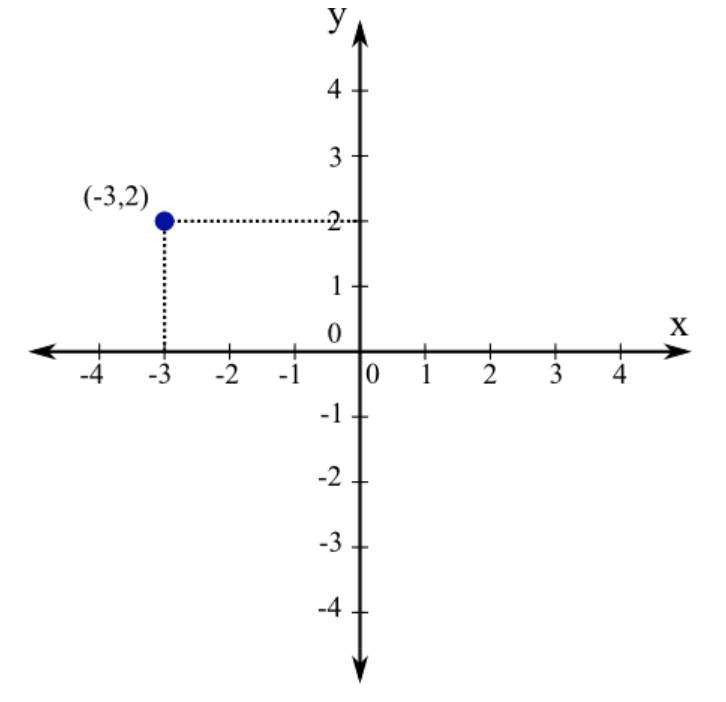
\includegraphics[scale=0.5]{Figures/appendixA_cartesian2D.png}
    \caption{Καρτεσιανές συντεταγμένες στο επίπεδο. Οι καρτεσιανές συντεταγμένες (x,y) του μπλε σημείου ορίζουν την θέση του σε σχέση με την αρχή των αξόνων, η οποία είναι η τομή των αξόνων x και y.}
    \label{fig:apxA_cartesian2D}
\end{figure}


\subsection{Καρτεσιανές συντεταγμένες στον χώρο}
Στον τριδιάστατο χώρο, το σύστημα των καρτεσιανών συντεταγμένων βασίζεται σε τρεις --κάθετους μεταξύ τους-- άξονες: τον άξονα x, τον άξονα y και τον άξονα z, όπως φαίνεται στο παρακάτω σχήμα. Οι τρεις άξονες τέμνονται σε ένα σημείο το οποίο αποτελεί την αρχή των αξόνων. Μπορεί κανείς να φανταστεί την αρχή των αξόνων στον τριδιάστατο χώρο ως το σημείο που τέμνονται οι τοίχοι και το πάτωμα σε μια γωνία ενός σπιτιού.
Ο άξονας x είναι η οριζόντια γραμμή κατά τη διεύθυνση της οποίας ο τοίχος στα αριστερά και το πάτωμα συναντιούνται. Ο άξονας y είναι η οριζόντια γραμμή κατά τη διεύθυνση της οποίας ο τοίχος στα δεξιά και το πάτωμα συναντιούνται. Τέλος, ο άξονας z είναι η κάθετη γραμμή κατά τη διεύθυνση της οποίας οι δύο τοίχοι ενώνονται.

\begin{figure}[h]
    \centering
    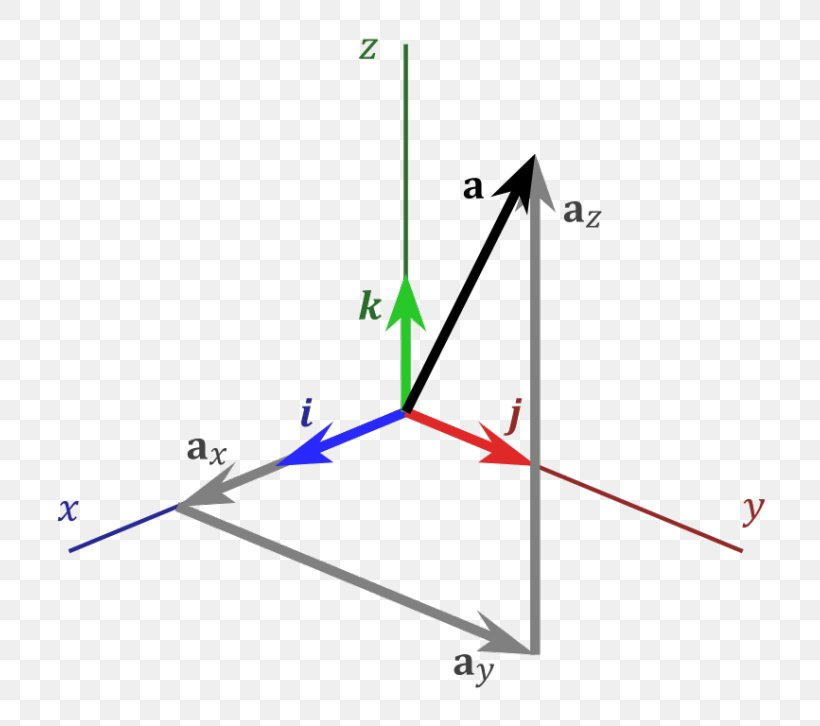
\includegraphics[scale=0.3]{Figures/appendixA_cartesian3D.jpg}
    \caption{Καρτεσιανές συντεταγμένες στον χώρο.}
    \label{fig:apxA_cartesian3D}
\end{figure}

Βάσει αυτών των ορισμών για τους θετικούς x, y και z άξονες, το σύστημα συντεταγμένων που προκύπτει ονομάζεται δεξιόστροφο και είναι σύμφωνο με τον κανόνα του δεξιού χεριού (ο αντίχειρας του δεξιού χεριού δείχνει προς την κατεύθυνση του θετικού άξονα z). Αλλάζοντας τις θέσεις των θετικών αξόνων x και y, κατασκευάζουμε το αριστερόστροφο σύστημα συντεταγμένων. Το δεξιόστροφο και αριστερόστροφο σύστημα συντεταγμένων αναπαριστούν δύο ισοδύναμα μαθηματικά συστήματα. Ιδιαίτερη προσοχή πρέπει να δίνεται όταν χρησιμοποιούμε το ένα σύστημα έναντι του άλλου καθώς η διαφορετική θεώρηση θα αλλάξει το πρόσημο σε κάποιες μαθηματικές σχέσεις. Γενικά, πάντως, το πιο σύνηθες είναι το δεξιόστροφο σύστημα.

Επιπρόσθετα των τριών αξόνων συντεταγμένων, συχνά αναφερόμαστε και σε τρία επίπεδα συντεταγμένων. Το επίπεδο xy είναι το οριζόντιο επίπεδο που ορίζεται από τους άξονες x και y. Είναι πανομοιότυπο με το διδιάστατο επίπεδο και αντιστοιχεί στο πάτωμα αν αναλογιστούμε το παράδειγμα του δωματίου που δώσαμε προηγουμένως. Παρόμοια, το επίπεδο xz είναι το κάθετο επίπεδο που ορίζεται από τους άξονες x και z, και αντιστοιχεί στον αριστερό τοίχο του παραδείγματος του δωματίου. Τέλος, το επίπεδο yz είναι το κάθετο επίπεδο που ορίζεται από τους άξονες y και z, και αντιστοιχεί στον δεξιό τοίχο του παραδείγματος του δωματίου. 
\\
{\color{red} \hrule}
Οι καρτεσιανές συντεταγμένες μπορούν να χρησιμοποιηθούν όχι μόνο για να ορίζουμε την θέση σημείων στο επίπεδο (ή στο χώρο), αλλά για να ορίσουμε και τις συνιστώσες διανυσμάτων. Οι καρτεσιανές συντεταγμένες διδιάστατων ή τριδιάστατων διανυσμάτων έχουν ακριβώς την ίδια μορφή με τις συντεταγμένες σημείων στο επίπεδο ή στον τριδιάστατο χώρο.

Από το σχήμα \ref{fig:apxA_cartesian3D} προκύπτει ότι το διάνυσμα θέσεως ,$\boldsymbol{a}$, θα δίνεται από τη σχέση: $$\boldsymbol{a} = a_x \boldsymbol{i} + a_y \boldsymbol{j} + a_z \boldsymbol{k}$$
Δεν υπάρχει λόγος να σταματήσει κανείς στις τρεις διαστάσεις. Μπορούμε να ορίσουμε διανύσματα σε τέσσερις, πέντε, ή και ακόμα υψηλότερες διαστάσεις απλά με το να ορίσουμε τέσσερα, πέντε ή περισσότερες καρτεσιανές συντεταγμένες. Δεν μπορούμε να οπτικοποιήσουμε, φυσικά, αυτές τις ανώτερες διαστάσεις, αλλά μπορούμε εύκολα να γράψουμε τη σειρά των αριθμών που αποτελούν τις συντεταγμένες.\\
{\color{red} \hrule}


\section{Πολικές συντεταγμένες}
Στις δύο διαστάσεις, οι καρτεσιανές συντεταγμένες (x,y) καθορίζουν τη θέση ενός σημείου P πάνω στο επίπεδο. Ένα διαφορετικό διδιάστατο σύστημα συντεταγμένων είναι το σύστημα των πολικών συντεταγμένων. Σε αυτό το σύστημα, αντί της χρήσης των αποστάσεων κατά μήκος δύο αξόνων για τον προσδιορισμό της θέσης του σημείου P στο επίπεδο, χρησιμοποιείται η απόσταση r από την αρχή των αξόνων και η γωνία $\theta$ που σχηματίζεται μεταξύ του ευθύγραμμου τμήματος που ενώνει το σημείο P με την αρχή των αξόνων και τον θετικό άξονα x. Οι πολικές συντεταγμένες (r, $\theta$) ενός σημείου P φαίνονται στο παρακάτω σχήμα (Σχήμα \ref{fig:apxA_polar_coordinates}).

\begin{figure}[h]
   \centering
\begin{subfigure}[h]{0.45\textwidth}
	\centering
   	 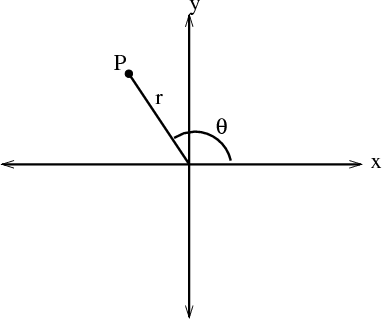
\includegraphics[width = \linewidth]{Figures/appendixA_polar_coordinates_whole.png} 
\end{subfigure}
\begin{subfigure}[h]{0.4\textwidth}
	\centering
	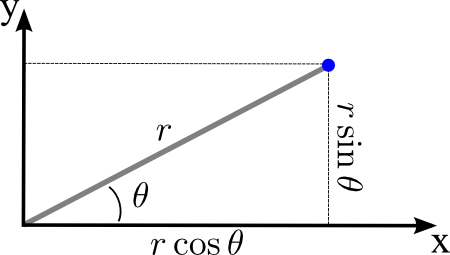
\includegraphics[width = \linewidth]{Figures/appendixA_polar_coordinates.png} 
    \end{subfigure}
    \caption{Πολικές συντεταγμένες στο επίπεδο.}
    \label{fig:apxA_polar_coordinates}
\end{figure}

Καθώς η παράμετρος r παίρνει τιμές από το μηδέν μέχρι το άπειρο, και η γωνία $\theta$ παίρνει τιμές από 0 έως $2\pi$, το σημείο P που ορίζεται από τις πολικές συντεταγμένες (r, $\theta$) καλύπτει κάθε πιθανό σημείο στο επίπεδο. Προσθέτοντας $2\pi$ στη γωνία $\theta$ επιστρέφουμε ξανά στο ίδιο σημείο από το οποίο ξεκινήσαμε, οπότε αν αφήσουμε τη γωνία $\theta$ να πάρει τιμές μεγαλύτερες του $2\pi$, κάθε σημείο θα είχε πολλαπλές πολικές συντεταγμένες. Άρα, περιορίζουμε το εύρος τιμών που μπορεί να πάρει η γωνία $\theta$ στο διάστημα $0 \leq \theta \leq 2\pi$. Όμως, παρόλα αυτά, ακόμα και με αυτόν τον περιορισμό, υπάρχει μια ιδιαιτερότητα στις πολικές συντεταγμένες: όταν $r=0$, το σημείο P βρίσκεται στην αρχή των αξόνων και είναι ανεξάρτητο της γωνίας $\theta$.

Μπορούμε να υπολογίσουμε τις καρτεσιανές συντεταγμένες ενός σημείου που δίνεται σε πολικές συντεταγμένες (r, $\theta$) φτιάχνοντας το τρίγωνο που φαίνεται στα δεξία του Σχήματος \ref{fig:apxA_polar_coordinates}.  
Η υποτείνουσα είναι το ευθύγραμμο τμήμα που ορίζεται από την αρχή των αξόνων και το σημείο ενδιαφέροντος, και το μήκος του είναι ίσο με r. Η προβολή αυτού του ευθύγραμμου τμήματος πάνω στον άξονα x είναι εκείνη η πλευρά του τριγώνου που είναι προσκείμενη στην γωνία $\theta$, έτσι ώστε $x=r \cos \theta$. Η y-συνιστώσα καθορίζεται από την κάθετη πλευρά, ώστε $y=r \sin \theta$. Οι σχέσεις μετασχηματισμού μεταξύ καρτεσιανών και πολικών συντεταγμένων δίνονται από:

\begin{eqnarray}
    x &=& r \cos \theta \\
    y &=& r \sin \theta 
\end{eqnarray}

Για τους αντίστροφους μετασχηματισμούς προκύπτει από τις παραπάνω σχέσεις ότι:
\begin{eqnarray}
    x^2 + y^2 &=& r^2 (\cos^2 \theta + \sin^2 \theta) = r^2 \Rightarrow r = \sqrt{x^2 + y^2} \\ \nonumber \\
    \frac{y}{x} &=& \frac{r \sin \theta}{r \cos \theta} = \tan \theta \Rightarrow \theta = \arctan \left( \frac{y}{x} \right)
\end{eqnarray}

Παρατηρούμε ότι με βάση τη σχέση Α.4 για το σημείο $(x,y) = (0,0)$, η γωνία $\theta$ δεν ορίζεται. Σε αυτή την περίπτωση όμως παίρνουμε ότι $\theta = 0$.


\section{Κυλινδρικές συντεταγμένες}
Οι κυλινδρικές συντεταγμένες είναι απλά μία προέκταση των διδιάστατων πολικών συντεταγμένων στις τρεις διαστάσεις. Πολύ απλά, συνδυάζουν τις πολικές συντεταγμένες στο επίπεδο xy με την συνηθισμένη z-συνιστώσα που συναντάμε στο καρτεσιανό σύστημα συντεταγμένων. Για να σχηματίσουμε το κυλινδρικό σύστημα συντεταγμένων ενός σημείου P, απλά προβάλουμε το εν λόγω σημείο σε ένα καινούργιο σημείο Q το οποίο βρίσκεται στο επίπεδο xy (Σχήμα \ref{fig:apxA_cylindrical_coordinates}). Στη συνέχεια, παίρνουμε τις πολικές συντεταγμένες (r, $\theta$) του σημείου Q, δηλαδή, r είναι η απόσταση του σημείου Q από την αρχή των αξόνων και $\theta$ η γωνία μεταξύ του θετικού άξονα x και του ευθύγραμμου τμήματος που ενώνει το σημείο Q με την αρχή των αξόνων. Η τρίτη κυλινδρική συντεταγμένη είναι ίδια με την συντεταγμένη z. Είναι, δηλαδή, η απόσταση του σημείου P από το επίπεδο xy (αρνητική τιμή σημαίνει ότι το σημείο P είναι κάτω από το επίπεδο xy). Το σχήμα που ακολουθεί αναπαριστά τις κυλινδρικές συντεταγμένες $(r, \theta, z)$ του σημειού P.

\begin{figure}[h]
    \centering
    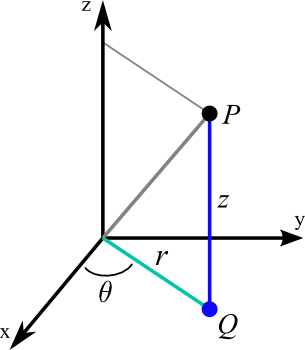
\includegraphics[scale=0.5]{Figures/appendixA_cylindrical_coordinates.png}
    \caption{Κυλινδρικές συντεταγμένες στον χώρο.}
    \label{fig:apxA_cylindrical_coordinates}
\end{figure}

Οι μετασχηματισμοί δίνονται από τις σχέσεις:
\begin{eqnarray}
    x &=& r \cos \theta \\
    y &=& r \sin \theta \\
    z &=& z
\end{eqnarray}
ενώ για τους αντίστροφους μετασχηματισμούς, ισχύουν οι σχέσεις Α.3 και Α.4.

\section{Σφαιρικές συντεταγμένες}
Οι σφαιρικές συντεταγμένες μπορεί να είναι αρχικά λίγο απαιτητικές ως προς την κατανόησή τους. Οι σφαιρικές συντεταγμένες καθορίζουν την θέση ενός σημειού στον τριδιάστατο χώρο, βάσει της απόστασης $\rho$ από την αρχή των αξόνων και δύο γωνιών $\theta$ και $\phi$. Αν κάποιος είναι εξοικιωμένος με τις πολικές συντεταγμένες, τότε η γωνία $\theta$ δεν είναι τόσο δύσκολο  να την κατανοήσει καθώς αποτελεί ουσιαστικά την ίδια γωνία $\theta$ που συναντάμε και στις πολικές συντεταγμένες. Γι' αυτό το λόγο αυτή η γωνία ονομάζεται και πολική γωνία. Μερικοί άνθρωποι όμως αντιμετωπίζουν κάποιες δυσκολίες όσον αφορά την κατανόηση της ύπαρξης της γωνίας $\phi$. Στη συνέχεια θα εξάγουμε τις σχέσεις μεταξύ Καρτεσιανών και σφαιρικών συντενταγμένων.

Οι σφαιρικές συντεταγμένες ορίζονται βάσει του σχήματος \ref{fig:apxA_spherical_coordinates}, το οποίο δείχνει τις σφαιρικές συντεταγμένες στο σημείο P.

\begin{figure}[h]
    \centering
    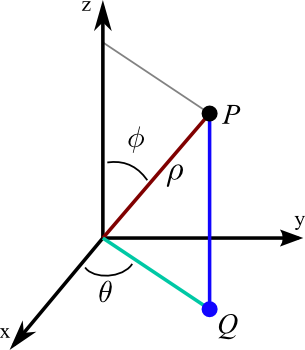
\includegraphics[scale=0.5]{Figures/appendixA_spherical_coordinates_simple.png}
    \caption{Σφαιρικές συντεταγμένες στον χώρο.}
    \label{fig:apxA_spherical_coordinates}
\end{figure}

Η συντεταγμένη $\rho$ είναι η απόσταση του σημείου P από την αρχή των αξόνων. Αν το σημείο Q είναι η προβολή του σημείου P πάνω στο επίπεδο xy, τότε $\theta$ είναι η γωνία μεταξύ του θετικού άξονα-x και του ευθύγραμμου τμήματος που ενώνει το σημείο Q με την αρχή των αξόνων. Τέλος, $\phi$ είναι η γωνία μεταξύ του θετικού άξονα-z και του ευθύγραμμου τμήματος που ενώνει το σημείο P με την αρχή των αξόνων και ονομάζεται αζιμούθια γωνία.

Μπορούμε να υπολογίσουμε τις σχέσεις που συνδέουν τις καρτεσιανές συντεταγμένες $(x,y,z)$ ενός σημείου P με τις σφαιρικές συντεταγμένες $(\rho, \theta, \phi)$ χρησιμοποιώντας βασική τριγωνομετρία. Το ροζ σκιασμένο τρίγωνο του Σχήματος \ref{fig:apxA_spherical_coordinates_derivation} έχει κορυφές την αρχή των αξόνων, το σημείο P και την προβολή αυτού του σημείου πάνω στον άξονα-z. Καθώς το μήκος της υποτείνουσας είναι $\rho$ και $\phi$ είναι η γωνία που σχηματίζει η υποτείνουσα με τον άξονα-z, η z-συνιστώσα του σημείου P (δηλαδή το ύψος του τριγώνου) είναι $z=\rho \cos \phi$. Το μήκος της άλλης πλευράς του τριγώνου είναι η απόσταση από το P μέχρι τον άξονα-z, η οποία είναι $r= \rho \sin \phi$. Η απόσταση του σημείου Q από την αρχή των αξόνων δίνεται από την ίδια σχέση.

\begin{figure}[h]
    \centering
    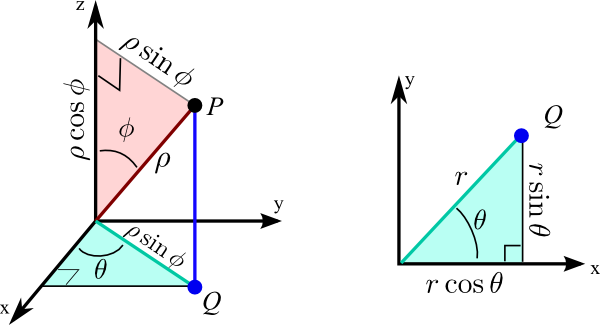
\includegraphics[scale=0.5]{Figures/appendixA_spherical_coordinates_analytical.png}
    \caption{Σχέση Καρτεσιανών και σφαιρικών συντενταγμένων.}
    \label{fig:apxA_spherical_coordinates_derivation}
\end{figure}

Το κυανό σκιασμένο τρίγωνο που φαίνεται και στο αρχικό τριδιάστατο σύστημα συντεταγμένων στα αριστερά, και στο επίπεδο xy στα δεξιά, είναι το τρίγωνο εκείνο του οποίου οι κορυφές είναι η αρχή των αξόνων, το σημείο Q, καθώς και η προβολή του πάνω στον άξονα-x. Στο δεξί σχήμα, η απόσταση του σημείου Q από την αρχή των αξόνων αποτελεί την υποτείνουσα του τριγώνου και συμβολίζεται με r. Με $\theta$ συμβολίζεται η γωνία που σχηματίζει η υποτείνουσα με τον άξονα-x. Οι x- και y-συνιστώσες του σημείου Q (που είναι οι ίδιες με τις x- και y-συνιστώσες του σημείου P) δίνονται από τις σχέσεις $x=r \cos \theta$ και $y=r \sin \theta$. Επειδή $r = \rho \sin \phi$, αυτές οι συνιστώσες μπορούν να γραφτούν και ως $x = \rho \sin \phi \cos \theta$ και $y = \rho \sin \phi \sin \theta$. Συνοπτικά, οι σχέσεις μετασχηματισμού μεταξύ καρτεσιανού και σφαιρικού συστήματος συντεταγμένων είναι:

\begin{eqnarray}
    x &=& \rho \sin \phi \cos \theta \\
    y &=& \rho \sin \phi \sin \theta \\
    z &=& \rho \cos \phi
\end{eqnarray}
όπου $\rho \geq 0, 0 \leq \theta \leq 2\pi, 0 \leq \phi \leq \pi$.

Δυστυχώς, η σύμβαση για τα σύμβολα που χρησιμοποιούνται στο σύστημα των σφαιρικών συντεταγμένων δεν είναι η ίδια σε όλα τα επιστημονικά πεδία. Για παράδειγμα, στη Φυσική, οι ρόλοι των γωνιών $\theta$ και $\phi$ είναι συνήθως ανεστραμμένοι, έτσι ώστε η γωνία $\theta$ να παριστάνει την αζιμούθια γωνία, και η γωνία $\phi$ την πολική. Προκειμένου να γίνει κατανοητή η χρήση των σφαιρικών συντεταγμένων, πρέπει πρώτα να ελέγξουμε ποια συμβατική ορολογία χρησιμοποιείται. Σε καμία περίπτωση δεν πρέπει να εννοείται ότι οποιαδήποτε χρήση σφαιρικών συντεταγμένων θα ακολουθεί την ίδια σύμβαση με αυτή που παρουσιάστηκε σε αυτό το Παράρτημα.
